\chapter{}
针对模型在复杂现实的泛化能力不足和数据多样性匮乏这两个问题,本章创新性地提出了一种毫米波雷达点云姿态识别的数据增强方法——$PointCloud PoseFusion$(PCPF)。该方法主要通过将特定的关键动作的点云数据定性提取并拼接到不同非关键动作点云场景中,以克服复杂场景点云数据难采集的问题,还可以增加点云数据多样性,以提升模型在复杂现实场景中的泛化能力。


\section{问题分析}
\section{PCPF毫米波雷达点云姿态识别数据增强方案}

\subsection{数据预处理}
%主要是数据预处理部分的公式推导,augment数据的公式
\subsection{PCPF数据增强算法}
%把python代码写成latex算法的格式



\section{实验设计和结果分析}
\subsection{实验评估指标}
\subsection{实验环境配置与训练参数设置}
\subsection{数据可视化分析}
\subsection{融合率与分段帧长对模型性能的影响}
% fusion_ratio: 20/30/40/50
% frame_len: 30/35/40/45/50/55/60
\begin{table}[htbp]
    \caption{融合率与分段帧长对模型性能的影响}
    \label{tab:fusion_frame_performance}
    \centering

    \begin{subtable}{\linewidth}
        \centering
        \caption{模型A的实验结果}
        \begin{tabular}{cc|cccc}
            \toprule
            融合率 (\%) & 分段帧长 & 准确率 (\%) & 精确率 & 召回率 & $F_1$分数 \\
            \midrule
            20 & 30 & 85.2 & 0.83 & 0.85 & 0.84 \\
            20 & 35 & 86.5 & 0.84 & 0.87 & 0.85 \\
            30 & 40 & 88.6 & 0.86 & 0.89 & 0.87 \\
            30 & 45 & 89.0 & 0.87 & 0.90 & 0.88 \\
            40 & 50 & 90.1 & 0.88 & 0.91 & 0.89 \\
            40 & 55 & 91.3 & 0.89 & 0.92 & 0.90 \\
            \bottomrule
        \end{tabular}
        \label{tab:modelA_performance}
    \end{subtable}

    \vspace{0.4cm} 

    \begin{subtable}{\linewidth}
        \centering
        \caption{模型B的实验结果}
        \begin{tabular}{cc|cccc}
            \toprule
            融合率 (\%) & 分段帧长 & 准确率 (\%) & 精确率 & 召回率 & $F_1$分数 \\
            \midrule
            20 & 30 & 84.0 & 0.82 & 0.83 & 0.82 \\
            20 & 35 & 85.5 & 0.83 & 0.86 & 0.84 \\
            30 & 40 & 87.0 & 0.85 & 0.88 & 0.86 \\
            30 & 45 & 88.5 & 0.86 & 0.89 & 0.87 \\
            40 & 50 & 89.8 & 0.87 & 0.90 & 0.88 \\
            40 & 55 & 90.5 & 0.88 & 0.91 & 0.89 \\
            \bottomrule
        \end{tabular}
        \label{tab:modelB_performance}
    \end{subtable}
\end{table}

% Second part of the table
\begin{table}[htbp]
    \ContinuedFloat
    \centering
    \begin{subtable}{\linewidth}
        \centering
        \caption{模型C的实验结果}
        \begin{tabular}{cc|cccc}
            \toprule
            融合率 (\%) & 分段帧长 & 准确率 (\%) & 精确率 & 召回率 & $F_1$分数 \\
            \midrule
            20 & 30 & 85.0 & 0.82 & 0.84 & 0.83 \\
            20 & 35 & 86.0 & 0.83 & 0.86 & 0.84 \\
            30 & 40 & 88.0 & 0.85 & 0.88 & 0.86 \\
            30 & 45 & 89.0 & 0.86 & 0.89 & 0.87 \\
            40 & 50 & 90.0 & 0.87 & 0.90 & 0.88 \\
            40 & 55 & 91.0 & 0.88 & 0.91 & 0.89 \\
            \bottomrule
        \end{tabular}
        \label{tab:modelC_performance}
    \end{subtable}

    \vspace{0.4cm}

    \begin{subtable}{\linewidth}
        \centering
        \caption{模型D的实验结果}
        \begin{tabular}{cc|cccc}
            \toprule
            融合率 (\%) & 分段帧长 & 准确率 (\%) & 精确率 & 召回率 & $F_1$分数 \\
            \midrule
            20 & 30 & 84.5 & 0.81 & 0.83 & 0.82 \\
            20 & 35 & 85.5 & 0.82 & 0.85 & 0.83 \\
            30 & 40 & 87.5 & 0.84 & 0.87 & 0.85 \\
            30 & 45 & 88.5 & 0.85 & 0.88 & 0.86 \\
            40 & 50 & 89.5 & 0.86 & 0.89 & 0.87 \\
            40 & 55 & 90.5 & 0.87 & 0.90 & 0.88 \\
            \bottomrule
        \end{tabular}
        \label{tab:modelD_performance}
    \end{subtable}

    \vspace{0.4cm}

    \begin{subtable}{\linewidth}
        \centering
        \caption{模型E的实验结果}
        \begin{tabular}{cc|cccc}
            \toprule
            融合率 (\%) & 分段帧长 & 准确率 (\%) & 精确率 & 召回率 & $F_1$分数 \\
            \midrule
            20 & 30 & 83.5 & 0.80 & 0.82 & 0.81 \\
            20 & 35 & 84.5 & 0.81 & 0.84 & 0.82 \\
            30 & 40 & 86.5 & 0.83 & 0.86 & 0.84 \\
            30 & 45 & 87.5 & 0.84 & 0.87 & 0.85 \\
            40 & 50 & 88.5 & 0.85 & 0.88 & 0.86 \\
            40 & 55 & 89.5 & 0.86 & 0.89 & 0.87 \\
            \bottomrule
        \end{tabular}
        \label{tab:modelE_performance}
    \end{subtable}

    \vspace{0.4cm}

    \begin{subtable}{\linewidth}
        \centering
        \caption{模型F的实验结果}
        \begin{tabular}{cc|cccc}
            \toprule
            融合率 (\%) & 分段帧长 & 准确率 (\%) & 精确率 & 召回率 & $F_1$分数 \\
            \midrule
            20 & 30 & 82.5 & 0.79 & 0.81 & 0.80 \\
            20 & 35 & 83.5 & 0.80 & 0.83 & 0.81 \\
            30 & 40 & 85.5 & 0.82 & 0.85 & 0.83 \\
            30 & 45 & 86.5 & 0.83 & 0.86 & 0.84 \\
            40 & 50 & 87.5 & 0.84 & 0.87 & 0.85 \\
            40 & 55 & 88.5 & 0.85 & 0.88 & 0.86 \\
            \bottomrule
        \end{tabular}
        \label{tab:modelF_performance}
    \end{subtable}
\end{table}



\subsection{采样方式对模型性能的影响}
%重复采样 vs 普通采样


\subsection{对比实验}
% 数据增强前后对比
%前后模型的评估指标对比(表格)

\begin{table}[htbp]
    \caption{模型数据增强前后指标对比}
    \label{tab:data augment metric-comparison}
    \centering

    \begin{subtable}{\linewidth}
        \centering
        \caption{模型数据增强前后准确率对比}
        \begin{tabular}{lccc}
            \toprule
            \textbf{模型} & \textbf{准确率前} & \textbf{准确率后} & \textbf{变化百分比} \\
            \midrule
            PointNet & 59.1\% & 64.1\% & +8.47\% \\
            PointNet++ & 88.6\% & 90.6\% & +2.26\% \\
            PointCNN & 88.4\% & 89.4\% & +1.13\% \\
            SpiderCNN & 90.6\% & 92.6\% & +2.21\% \\
            DGCNN & 93.1\% & 94.1\% & +1.07\% \\
            RsNet & 92.1\% & 93.1\% & +1.09\% \\
            MR-PPFN PointNet-BiLSTM & 88.6\% & 89.6\% & +1.13\% \\
            MR-PPFN PointNet++-BiLSTM & 88.6\% & 90.6\% & +2.26\% \\
            MR-PPFN PointCNN-BiLSTM & 88.4\% & 89.4\% & +1.13\% \\
            MR-PPFN SpiderCNN-BiLSTM & 90.6\% & 92.6\% & +2.21\% \\
            MR-PPFN DGCNN-BiLSTM & 92.3\% & 93.3\% & +1.08\% \\
            MR-PPFN RsNet-BiLSTM & 92.3\% & 93.3\% & +1.08\% \\
            \bottomrule
        \end{tabular}
        \label{tab:data augment accuracy-comparison}
    \end{subtable}

    \vspace{0.4cm}

    \begin{subtable}{\linewidth}
        \centering
        \caption{模型数据增强前后精确率对比}
        \begin{tabular}{lccc}
            \toprule
            \textbf{模型} & \textbf{精确率前} & \textbf{精确率后} & \textbf{变化百分比} \\
            \midrule
            PointNet & 55.0\% & 60.0\% & +9.09\% \\
            PointNet++ & 87.0\% & 89.0\% & +2.30\% \\
            PointCNN & 86.5\% & 87.5\% & +1.16\% \\
            SpiderCNN & 89.0\% & 91.0\% & +2.25\% \\
            DGCNN & 92.0\% & 93.0\% & +1.09\% \\
            RsNet & 91.0\% & 92.0\% & +1.10\% \\
            MR-PPFN PointNet-BiLSTM & 87.0\% & 88.0\% & +1.15\% \\
            MR-PPFN PointNet++-BiLSTM & 87.0\% & 89.0\% & +2.30\% \\
            MR-PPFN PointCNN-BiLSTM & 86.5\% & 87.5\% & +1.16\% \\
            MR-PPFN SpiderCNN-BiLSTM & 89.0\% & 91.0\% & +2.25\% \\
            MR-PPFN DGCNN-BiLSTM & 91.5\% & 92.5\% & +1.09\% \\
            MR-PPFN RsNet-BiLSTM & 91.5\% & 92.5\% & +1.09\% \\
            \bottomrule
        \end{tabular}
        \label{tab:data augment  precision-comparison}
    \end{subtable}
\end{table}

\begin{table}[htbp]
    \ContinuedFloat
    \centering

    \begin{subtable}{\linewidth}
        \centering
        \caption{模型数据增强前后召回率对比}
        \begin{tabular}{lccc}
            \toprule
            \textbf{模型} & \textbf{召回率前} & \textbf{召回率后} & \textbf{变化百分比} \\
            \midrule
            PointNet & 54.0\% & 59.0\% & +9.26\% \\
            PointNet++ & 86.0\% & 88.0\% & +2.33\% \\
            PointCNN & 85.5\% & 86.5\% & +1.17\% \\
            SpiderCNN & 88.0\% & 90.0\% & +2.27\% \\
            DGCNN & 91.0\% & 92.0\% & +1.10\% \\
            RsNet & 90.0\% & 91.0\% & +1.11\% \\
            MR-PPFN PointNet-BiLSTM & 86.0\% & 87.0\% & +1.16\% \\
            MR-PPFN PointNet++-BiLSTM & 86.0\% & 88.0\% & +2.33\% \\
            MR-PPFN PointCNN-BiLSTM & 85.5\% & 86.5\% & +1.17\% \\
            MR-PPFN SpiderCNN-BiLSTM & 88.0\% & 90.0\% & +2.27\% \\
            MR-PPFN DGCNN-BiLSTM & 90.5\% & 91.5\% & +1.11\% \\
            MR-PPFN RsNet-BiLSTM & 90.5\% & 91.5\% & +1.11\% \\
            \bottomrule
        \end{tabular}
        \label{tab:data augment recall-comparison}
    \end{subtable}

    \vspace{0.4cm}

    \begin{subtable}{\linewidth}
        \centering
        \caption{模型数据增强前后F1分数对比}
        \begin{tabular}{lccc}
            \toprule
            \textbf{模型} & \textbf{F1分数前} & \textbf{F1分数后} & \textbf{变化百分比} \\
            \midrule
            PointNet & 54.5\% & 59.5\% & +9.17\% \\
            PointNet++ & 86.5\% & 88.5\% & +2.31\% \\
            PointCNN & 86.0\% & 87.0\% & +1.16\% \\
            SpiderCNN & 88.5\% & 90.5\% & +2.26\% \\
            DGCNN & 91.5\% & 92.5\% & +1.09\% \\
            RsNet & 90.5\% & 91.5\% & +1.10\% \\
            MR-PPFN PointNet-BiLSTM & 86.5\% & 87.5\% & +1.16\% \\
            MR-PPFN PointNet++-BiLSTM & 86.5\% & 88.5\% & +2.31\% \\
            MR-PPFN PointCNN-BiLSTM & 86.0\% & 87.0\% & +1.16\% \\
            MR-PPFN SpiderCNN-BiLSTM & 88.5\% & 90.5\% & +2.26\% \\
            MR-PPFN DGCNN-BiLSTM & 91.0\% & 92.0\% & +1.10\% \\
            MR-PPFN RsNet-BiLSTM & 91.0\% & 92.0\% & +1.10\% \\
            \bottomrule
        \end{tabular}
        \label{tab:data augment f1-comparison}
    \end{subtable}
\end{table}
 
%前后的模型的准确率的条状对比图
%前后数据量的对比(条状图)

\begin{figure}[htbp]
    \centering
    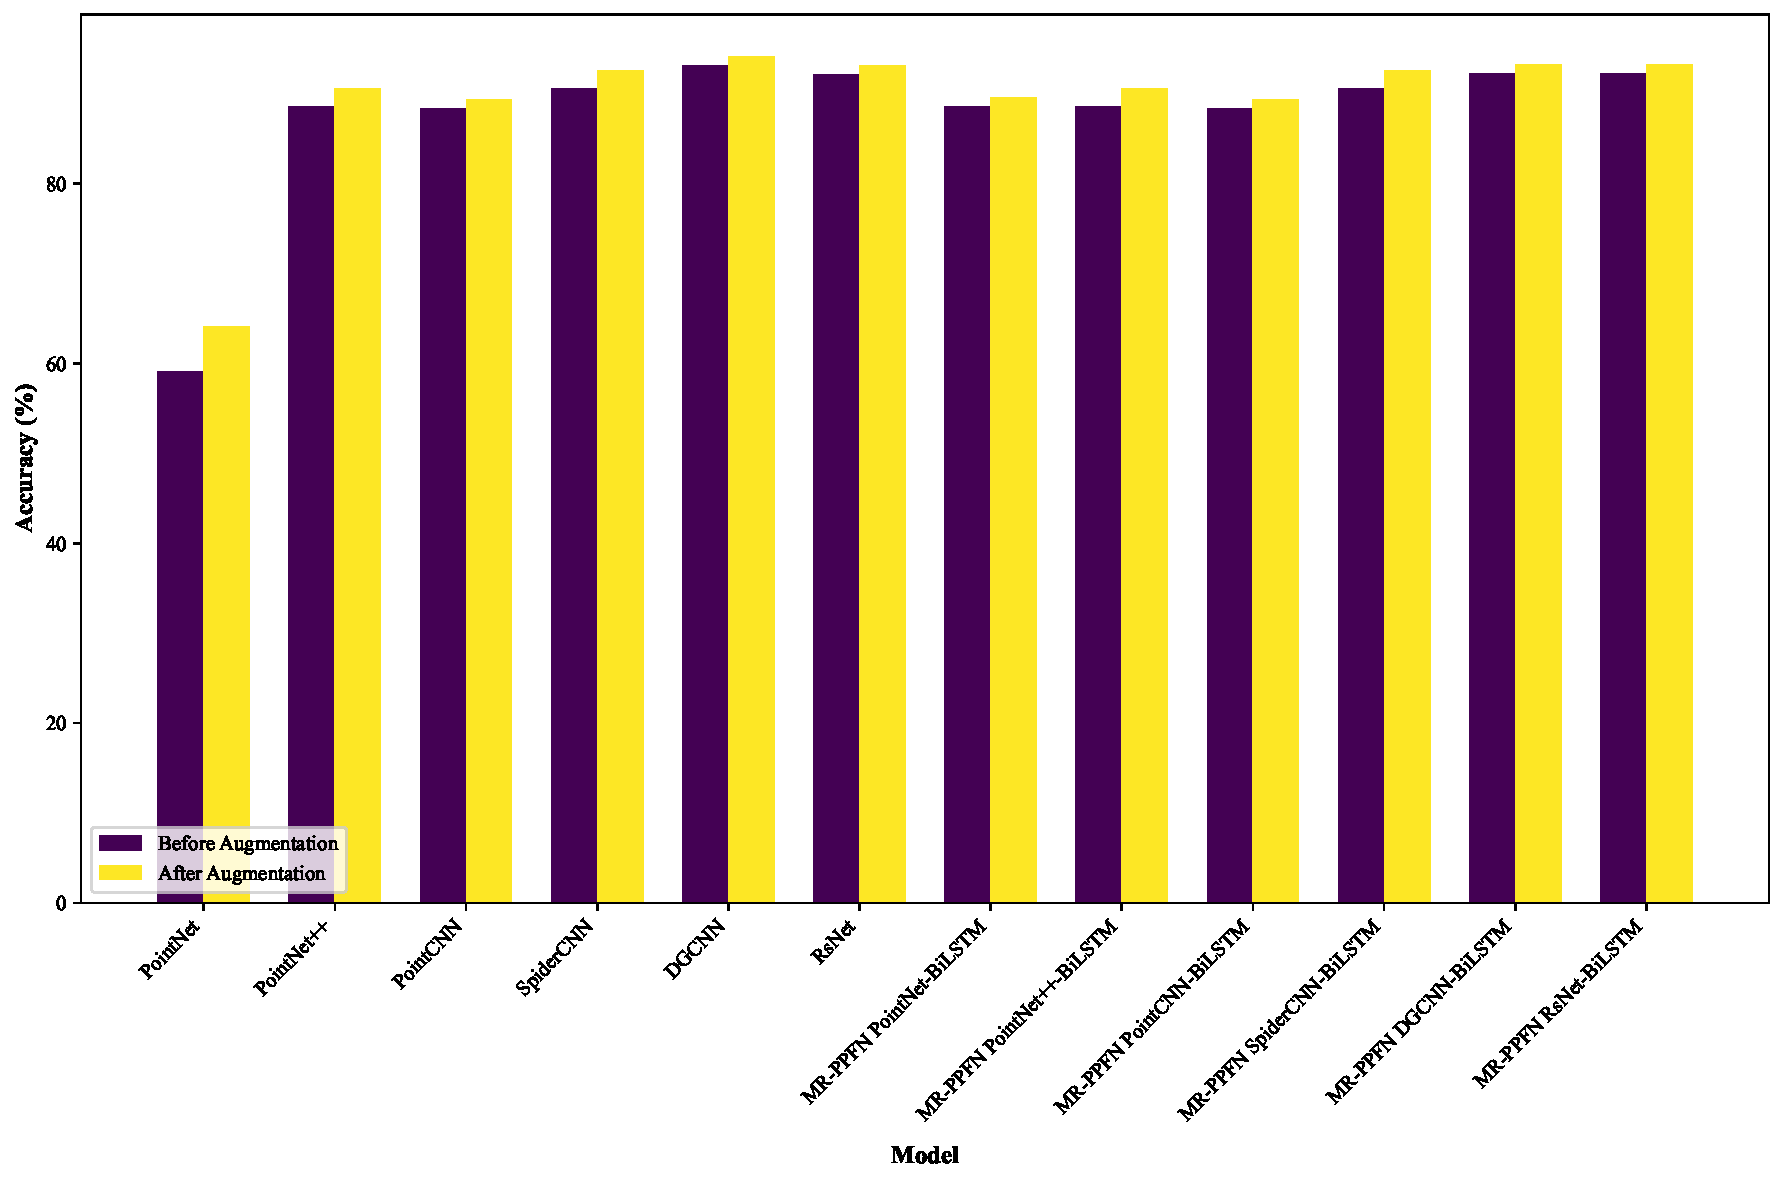
\includegraphics[width=1\linewidth]{imgs/data_augment_accuracy_comparison.pdf}
    \caption{数据增强前后准确率对比图}
    \label{fig:data_augment_accuracy_comparison_bar_chart}
\end{figure}

\begin{figure}[htbp]
    \centering
    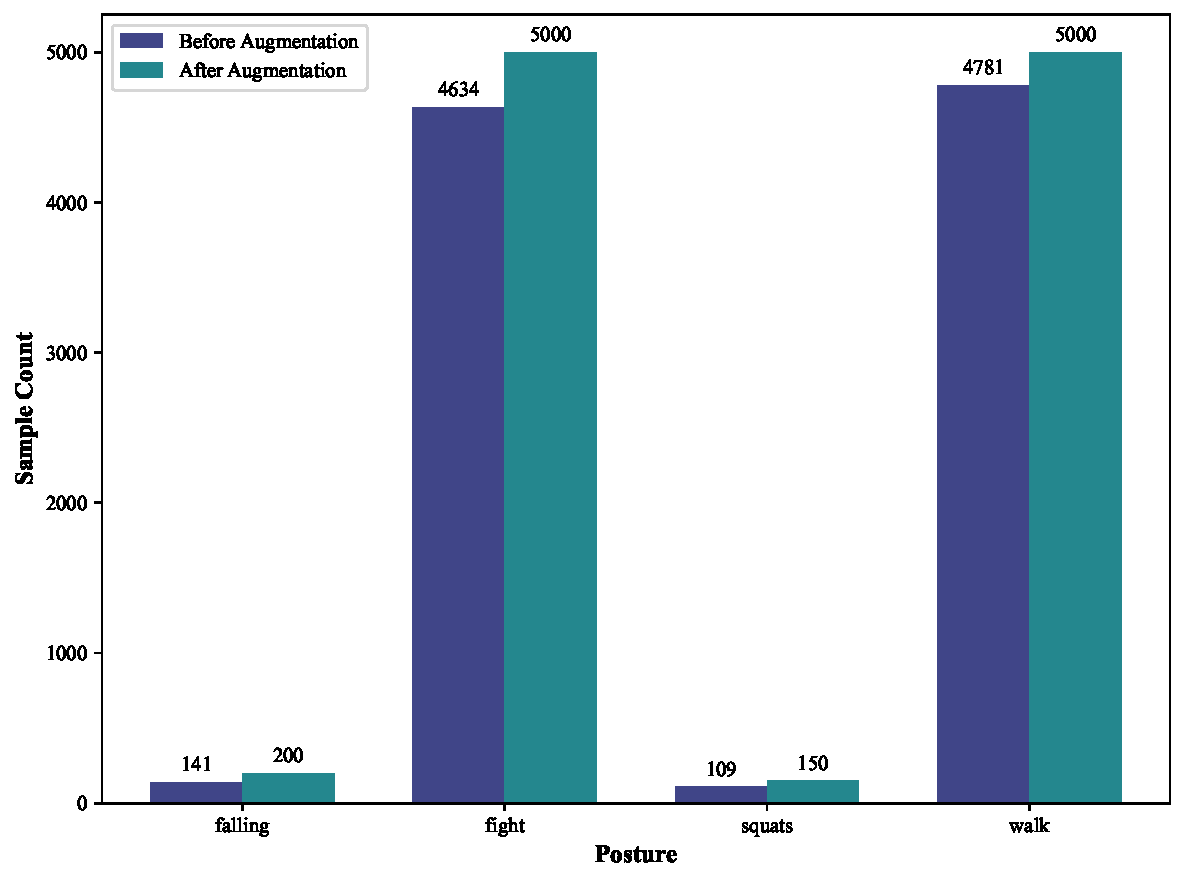
\includegraphics[width=1\linewidth]{imgs/data_augment_sample_quantities_comparison.pdf}
    \caption{数据增强前后样本数量对比图}
    \label{fig:data_augment_sample_quantities_comparison_bar_chart}
\end{figure}

